\documentclass[../main.tex]{subfiles}
\begin{document}

\begin{figure}[t]
\centering
    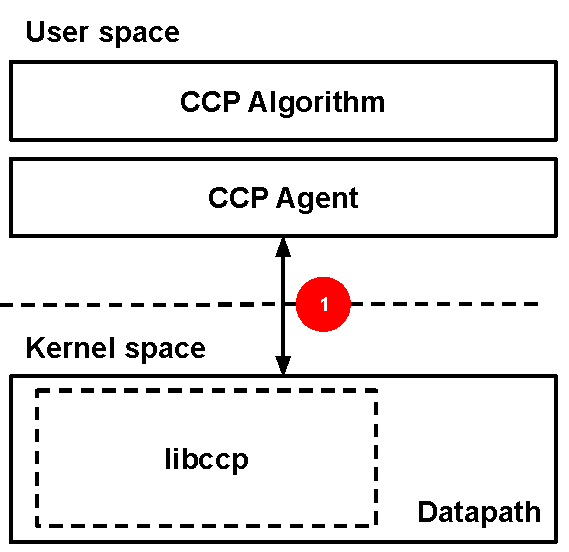
\includegraphics[width=\columnwidth]{img/ccp-traditional}
    \caption{CCP's conventional Linux kernel datapath, implemented as a kernel module, utilizes \texttt{libccp} to communicate with the CCP agent.
        Communication (1) is accomplished via Netlink sockets or a custom character device.
    }\label{fig:ccptraditional}
\end{figure}

Figure~\ref{fig:ccptraditional} illustrates the current CCP stack.
Notably, the CCP algorithm and agent both run in user space, while the datapath is implemented and run completely in kernel space.
Conventionally, CCP datapath program implementations such as Linux kernel's TCP stack, mTCP, and Google's QUIC all utilize \texttt{libccp} to interface with the CCP agent (Portus) \cite{ccp}.

\subsection{eBPF Implementation}

Due to eBPF's intense verifier requirements and stipulations, running \texttt{libccp} within the eBPF program was deemed difficult.
Consequently, we create a user space layer between the CCP agent and the Linux kernel's TCP stack, called eBPFCCP.

eBPFCCP is written in Rust and runs \texttt{libccp} in user space to communicate with the CCP agent while also managing and communicating with the eBPF-based datapath program.
eBPFCCP's role is to collect primitive congestion signals from the eBPF program, send them over to the CCP agent, and execute instructions sent by the CCP agent to influence TCP behavior.
As shown in Figure~\ref{fig:ebpfccp}, eBPFCCP communicates with the CCP agent via Unix-domain sockets as its IPC mechanism and interfaces with the eBPF datapath program through BPF hash maps and BPF ring buffers.

\begin{figure}[t]
\centering
    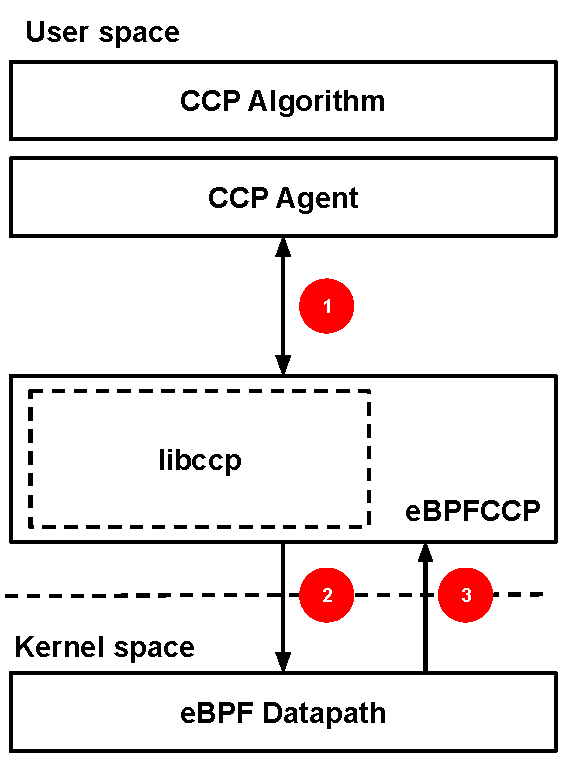
\includegraphics[width=\columnwidth]{img/ebpfccp}
    \caption{The eBPFCCP stack runs \texttt{libccp} in user space, communicating (1) with the CCP agent via Unix-domain sockets and interfacing with the eBPF datapath program via (2) BPF hash maps and (3) BPF ring buffers.
    }\label{fig:ebpfccp}
\end{figure}

On the eBPF datapath side, we use eBPF's \texttt{struct\_ops} API to attach congestion control-specific hooks to the TCP stack.
Each of these hooks operate on a per-flow basis.
When a new flow is created, the eBPF datapath program records the flow's information in a BPF ring buffer called \texttt{create\_conn\_events}.
This signals eBPFCCP to retrieve the new flow's information and pass it to the CCP agent.
Similarly, when a flow is terminated, the eBPF datapath program writes an event to the \texttt{free\_conn\_events} ring buffer, which eBPFCCP then reads to perform flow cleanup actions.
As new ACKs arrive, the eBPF datapath program reads the TCP state and calculates primitive congestion signals, which are then written to the \texttt{signals} ring buffer, read by eBPFCCP, and sent to the CCP agent.
Then, messages pertaining to congestion window size and sending rate are written to the \texttt{connections} hash map.
The BPF maps used by the eBPF datapath and eBPFCCP are summarized in Table~\ref{tab:maptable}.

\begin{table}[htbp]
    \centering
    \footnotesize
    \begin{tabular}{@{}p{0.35\columnwidth} p{0.5\columnwidth}@{}}
        \toprule
        \textbf{Map} & \textbf{Description} \\[3pt]
        \midrule
        \texttt{connections} (BPF Hash) &
        eBPFCCP writes per-flow congestion window size and pacing rate. 
        The eBPF datapath reads these values and updates the TCP state accordingly. \\[6pt]
        
        \texttt{signals} (BPF Ringbuf) &
        The eBPF datapath writes primitive signal measurements into this buffer. 
        The eBPFCCP reads these measurements and forwards them to the CCP agent. \\[6pt]
        
        \texttt{create\_conn\_events} (BPF Ringbuf) &
        Whenever a new flow is created, the eBPF datapath records flow information here. 
        The eBPFCCP then retrieves and passes these details to the CCP agent. \\[6pt]
        
        \texttt{free\_conn\_events} (BPF Ringbuf) &
        Upon flow termination, the eBPF datapath writes an event. 
        The eBPFCCP reads and relays this information to the CCP agent for flow cleanup actions. \\[3pt]
        \bottomrule
    \end{tabular}
    \caption{BPF Maps used by the eBPF datapath and eBPFCCP for managing flow states, signals, and events.}
    \label{tab:maptable}
\end{table}

Overall, eBPFCCP aims to act as a bridge between the CCP agent and the eBPF datapath program.

\end{document}
